\section{Interpolation artifacts and outlier position distribution}



\begin{figure}[t]
  \centering
  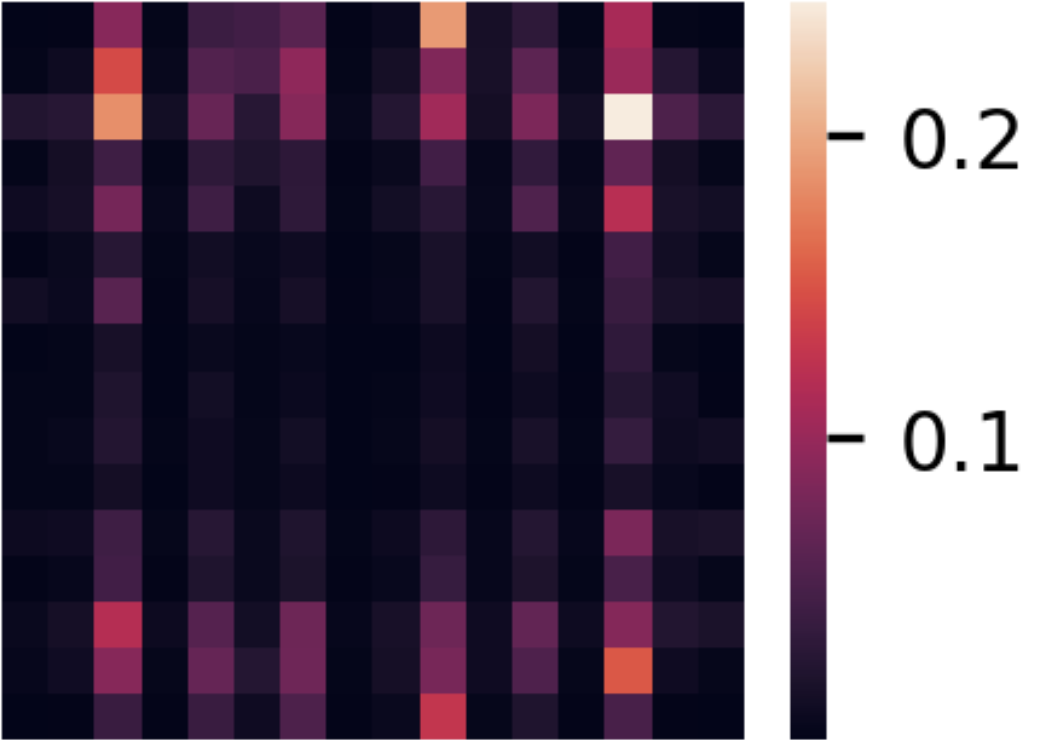
\includegraphics[width=0.3\textwidth]{resources/230918_interp_artifacts/aliased.png}
  \hspace{0.1\textwidth}
  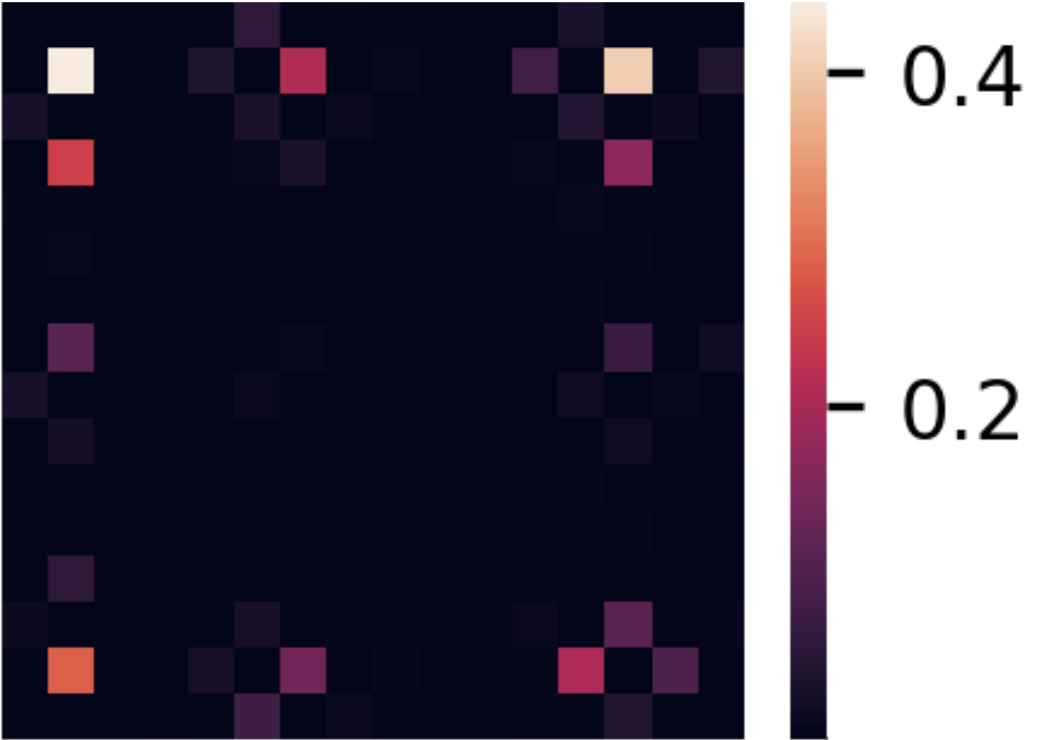
\includegraphics[width=0.3\textwidth]{resources/230918_interp_artifacts/antialiased.png}
  \caption{
    Feature norms along locations: proportion of tokens with norm larger than the cutoff value at a given location. Left: official DINOv2 model (no antialiasing), right: our models (with antialiasing).
    At some positions, more than 20\% of tokens have a high norm.
  }
  \label{fig:outlier_positions}
\end{figure}


\begin{figure}[t]
  \centering
  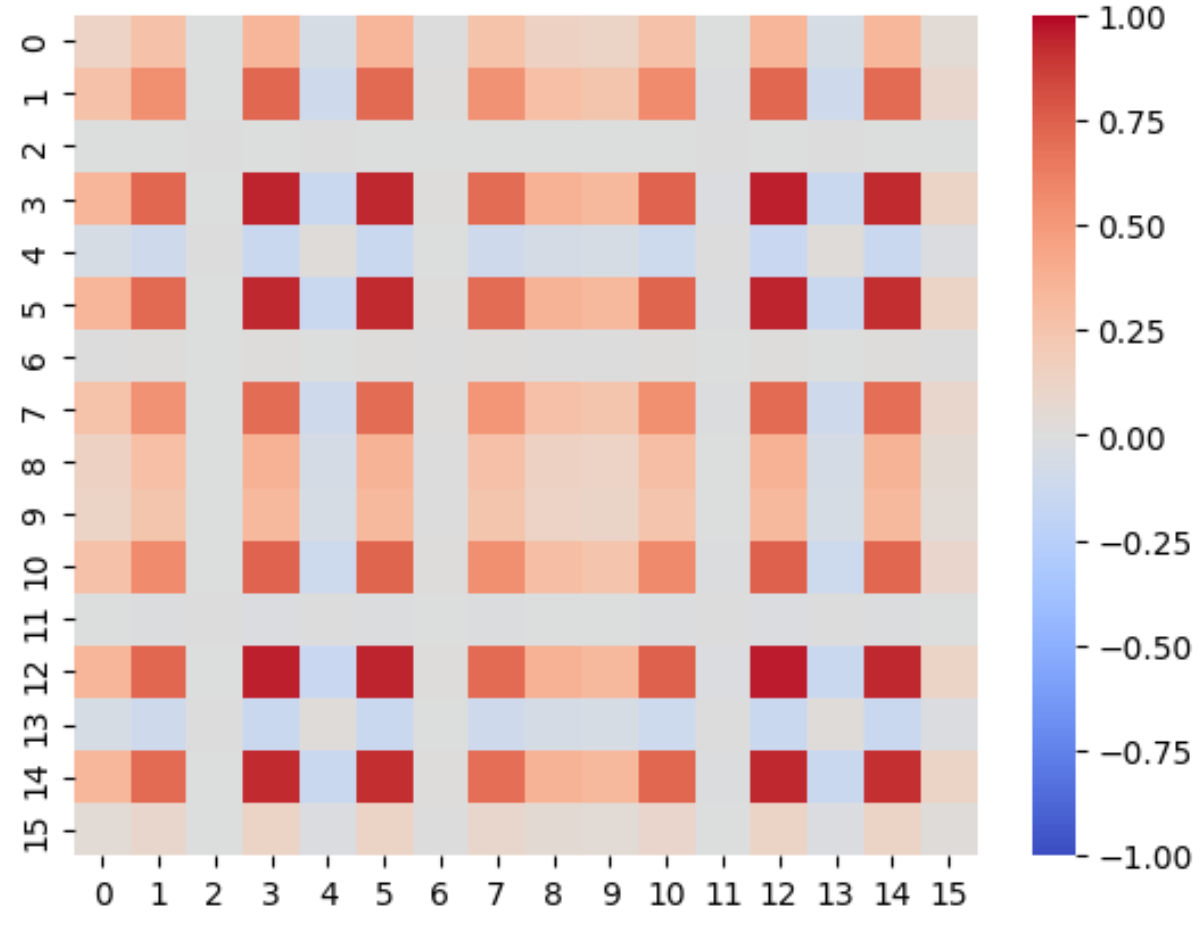
\includegraphics[width=0.4\textwidth]{resources/230918_interp_artifacts/interp_artifacts.png}
  \caption{
    Propagating unit gradients through a bicubic interpolation ($16\times16 \rightarrow 7\times7$) without antialiasing. We observe a striping pattern similar to the one of Fig. \ref{fig:outlier_positions} (left).
  }
  \label{fig:interp_gradient_stripes}
\end{figure}



We plot in Figure \ref{fig:outlier_positions} (left) the proportion of outlier tokens, characterized by a norm larger than the cutoff value defined manually, following the distribution of norms shown in Fig. \ref{fig:norms_hist} (main text). We make two observations: 

First, the distribution has a vertical-striped pattern. We investigate this phenomenon and notice that in the original DINOv2 implementation, during training the position embeddings are interpolated from a $16\times16$ map into a $7\times7$ map, without antialiasing. Propagating unit gradients through such an interpolation function (bicubic resize) leads to the following gradients, shown in Fig. \ref{fig:interp_gradient_stripes}. 
In this work, when producing results with DINOv2 (especially for the results in Tables \ref{tab:linear},\ref{tab:lost}), we always apply antialiasing in the interpolation operator, removing the striping pattern, which gives an updated distribution of outlier positions as shown in Fig. \ref{fig:outlier_positions} (right).

Second, the outliers tend to appear in areas closer to the border of the feature map rather than in the center. Our interpretation is that the base model tends to recycle tokens in low-informative areas to use as registers: pictures produced by people tend to be object-centric, and in this case the border areas often correspond to background, which contains less information than the center.


\section{Complexity analysis}

\begin{figure}[t]
  \centering
  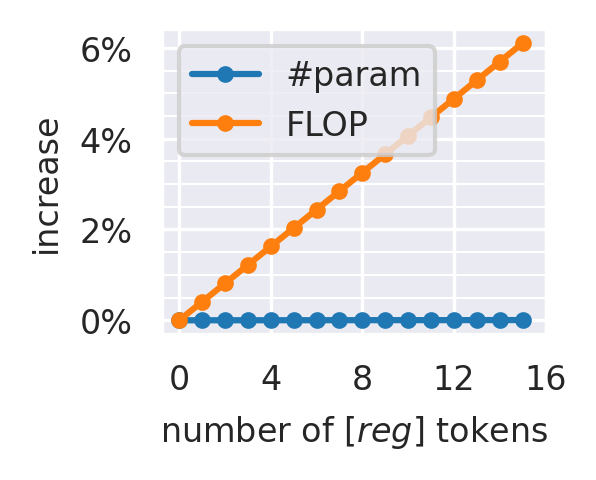
\includegraphics[width=0.3\textwidth]{resources/23098_param_flop_vs_n_reg.png}
  \caption{
    Increase in model parameter and FLOP count when adding different numbers of registers.
    Adding registers can increase model FLOP count by up to 6\% for 16 registers.
    However, in the more common case of using 4 registers, that we use in most of our experiments, this increase is below 2\%.
    In all cases, the increase in model parameters is negligible.
  }
  \label{fig:param_flop_vs_n_reg}
\end{figure}


Since our proposed fix introduces new tokens, it also increases the number of learnable parameters and the FLOP count of the model. We show in Fig. \ref{fig:param_flop_vs_n_reg} the relationship between number of registers and increase in model FLOP count and parameter count. We observe that adding registers induces a negligible change in number of parameters, and a slight change in FLOP count. Still, for $n=4$ registers, the increase in FLOPs stays below 2\%.


\section{Analysis of LOST performance}
\label{sec:appendix-lost}
The results presented in Sec.~\ref{sec:obj_discovery} show that adding registers allows us to obtain better object discovery performance with DINOv2 models.
The conclusions for the two other models studied in this work could be more crisp.
In order to understand why this is so, we qualitatively study the impact of removing artifacts on the intermediate computations in the LOST algorithm.
We show the intermediate outputs of LOST for all models on a given input image in Fig.~\ref{fig:lost-qualitative}.

Adding registers improves the scores and the resulting seed expansion for DeiT-III and DINOv2. 
This observation is coherent with the improved numbers reported in Table~\ref{tab:lost}.
For OpenCLIP, however, the LOST algorithm seems robust to the type of outliers observed in the local features.
Adding registers does remove artifacts (as clearly shown in Fig.~\ref{fig:supmat_pagefig_pca_beforeafter}) but does not have much impact on the LOST score.
It is also worth noting that OpenCLIP, with or without registers, provides comparable performance to DINOv2 without registers and DeiT-III with registers.
The qualitative assessment is coherent with the numbers reported in Table~\ref{tab:lost}.

\begin{figure}[t]
  \centering
  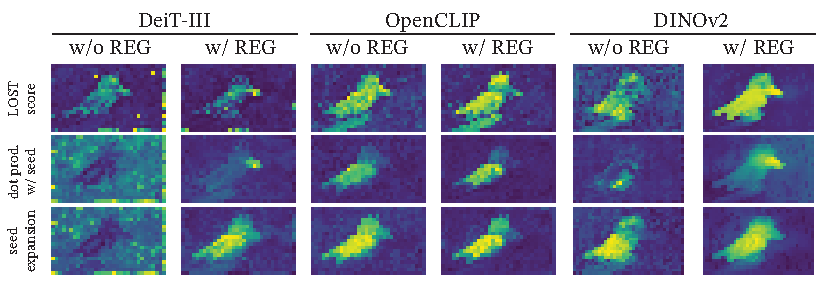
\includegraphics[width=\linewidth]{resources/lost-qualitative.pdf}
  \caption{
    \new{
        Illustration of the intermediate computations in the LOST algorithm for all models.
        Adding registers drastically improves the look of all intermediate steps for DeiT-III and DINOv2.
        The difference is less striking for the OpenCLIP model.
    }
  }
  \label{fig:lost-qualitative}
\end{figure}

A surprising observation is that despite the existence of high-norm patches in the output of OpenCLIP models without registers (as seen in Fig.~\ref{fig:norm_distrib_before_after}), the seed expansion score in Fig.~\ref{fig:lost-qualitative} looks smooth.
In the LOST experiment with OpenCLIP models, we do not use the features directly, but the values from the computation of attention maps. 
In Fig.~\ref{fig:lost-qualitative-clip}, we show the seed expansion score for OpenCLIP models with and without registers for keys, queries and values. 
We see that artifacts are clearly visible as spots in the background for keys and queries, for the model without registers.
As soon as registers are used, the LOST score is focusing on the object, with a smoother score for values.
We qualitatively observe that for the OpenCLIP model, the value projection filters out the outliers even without registers. This means that the outliers appear to live in the null space of the value projection layer; the investigation for this phenomenon is left for future work.

\begin{figure}[t]
  \centering
  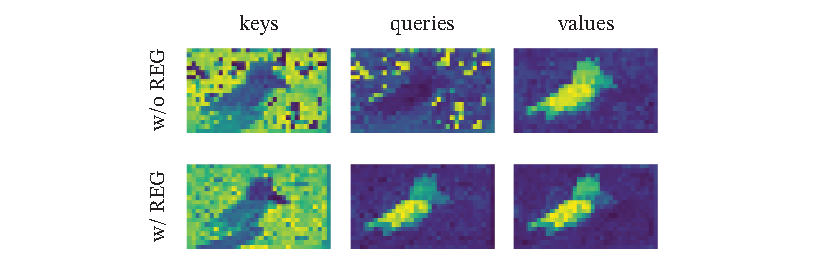
\includegraphics[width=\linewidth]{resources/lost-qualitative-clip-qkv.pdf}
  \caption{
    Illustration of the seed expansion score in LOST for an OpenCLIP model with and without registers for the three types of features considered: keys, queries, and values.
    The score is qualitatively improved across all features, with fewer artifacts appearing. 
    Interestingly, the seed expansion map computed using values does not exhibit artifacts with nor without registers.
  }
  \label{fig:lost-qualitative-clip}
\end{figure}



\section{Behavior of models trained with registers}
In order to better understand the phenomenon at hand, we examine the question of to what extent did the register tokens "replace" the high-norm tokens and took on the same role.
\subsection{Norms}
\begin{figure}[h]
  \centering
  \begin{subfigure}[b]{0.3\textwidth}
      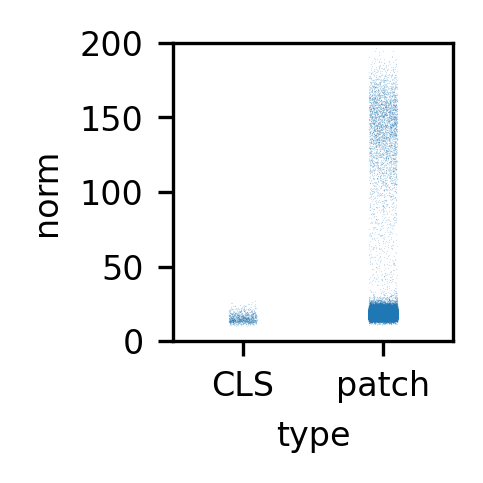
\includegraphics[width=\linewidth]{resources/231120_fig_norm_distrib_vs_token_type_dinov2_0reg.png}
      \caption{DINOv2 - no register}
      \label{fig:wertghjrewq}
   \end{subfigure}
   \hfill
  \begin{subfigure}[b]{0.6\textwidth}
      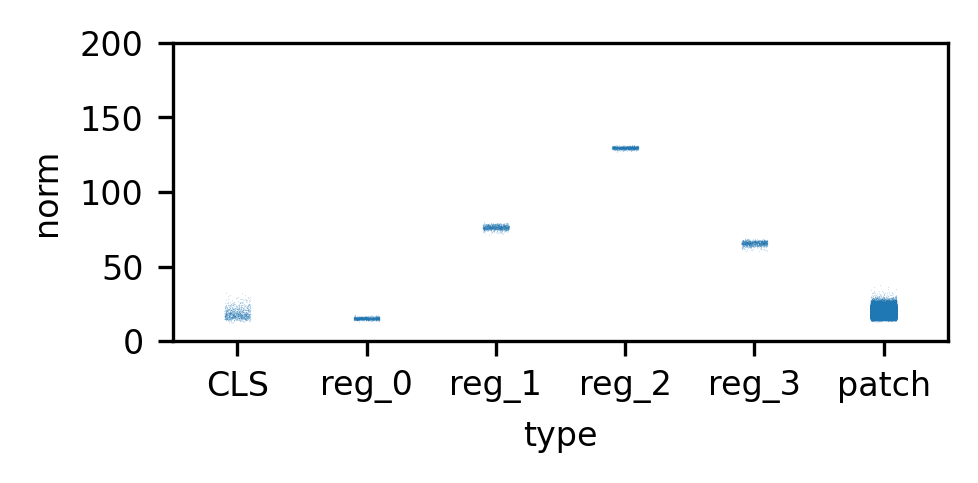
\includegraphics[width=\linewidth]{resources/231120_fig_norm_distrib_vs_token_type_dinov2_4reg.png}
      \caption{DINOv2 - 4 registers}
      \label{fig:wertghjrewhjtyr}
   \end{subfigure}
  
  \caption{
  Distribution of token norms for a DINOv2 model without (left) and with (right) 4 registers. Introducing registers entirely negates the high-norm outliers among the patch tokens. 
  }
  \label{fig:register_norm_distrib}
\end{figure}

In Fig. \ref{fig:register_norm_distrib} we compare the distribution of token norms for a model with or without registers. This figure is similar to Fig. \ref{fig:norm_distrib_before_after} but with a finer granularity, as we also plot the norm distribution of individual register tokens and \texttt{[CLS]} tokens. We observe the following: with registers, the norms of patch tokens do not contain outliers anymore, and the high-norm tokens are entirely contained in the set of registers. As a result, we conclude that the behavior leading to high-norm outliers in the model is effectively absorbed in the registers.

An additional interesting observation is that the norms of the registers appear to be quantized, compared to the previous outliers; we leave the investigation of this phenomenon for future work.

\subsection{Information held by tokens}
We report on table \ref{tab:classif_logreg_token_types-acc} the linear probing performance of models trained with and without registers, when using different tokens as representations. We evaluate on the aircrafts dataset, as it showed clear conclusions in the similar table \ref{tab:logreg_weird_patches_image_classif}. We observe that adding a register does not significantly modify the scores obtained with the \texttt{[CLS]} or patch tokens. However, the outlier patches are removed, and their behavior is transferred to the newly added register.

\begin{table}[h]
    \centering
    \begin{tabular}{ccccc}
         \toprule
            & \multicolumn{4}{c}{top-1 accuracy} \\
         \#registers & \texttt{[CLS]} & normal patch & outlier patch & register \\
         \midrule
         0 & 84.6 & 15.5 & 73.3 & N/A \\
         1 & 85.2 & 14.5 & N/A & 71.1 \\
         \bottomrule
    \end{tabular}
    \caption{Linear probing of models with and without registers on the Aircraft dataset, using various tokens as representation. We observe that the behavior of the outlier tokens, aggregating global information, is absorbed into the register.}
    \label{tab:classif_logreg_token_types-acc}
\end{table}

We further conduct an evaluation of the local information contained in the patch tokens of a model trained with and without registers (table \ref{tab:classif_logreg_token_types-pos}). We observe that the non-outliers patches, in both cases, hold similar local information, confirming that the registers only remove the outlier behavior, without significantly modifying the information held by the other patches.




\begin{table}[h]
    \centering
    \begin{tabular}{cccc}
         \toprule
          & & position prediction & reconstruction \\
         \#registers& patches considered & top-1 acc & L2 error $\downarrow$ \\
         \midrule
         0 & non-outliers & 66.3 & 15.9  \\
         4 & non-outliers (ie all) & 65.8 & 16.0  \\
        \bottomrule
    \end{tabular}
    \caption{Linear probing for local information on the patch tokens of models trained without or with registers. We only consider patches considered "normal", i.e. not the high-norm outliers. We observe that adding registers does not significantly modify the scores of these patches.}
    \label{tab:classif_logreg_token_types-pos}
\end{table}


\subsection{Positional focus}
\begin{figure}[h]
  \centering
  \begin{subfigure}[b]{0.15\textwidth}
      
\includegraphics[width=\linewidth]{resources/231121_average_attn_location_cls.png}
      \caption{\texttt{[CLS]}}
   \end{subfigure}
   \hfill
  \begin{subfigure}[b]{0.15\textwidth}
      
\includegraphics[width=\linewidth]{resources/231121_average_attn_location_reg0.png}
      \caption{reg$_0$}
   \end{subfigure}
   \hfill
  \begin{subfigure}[b]{0.15\textwidth}
      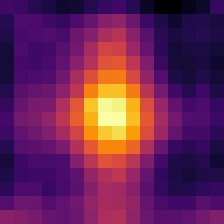
\includegraphics[width=\linewidth]{resources/231121_average_attn_location_reg1.png}
      \caption{reg$_1$}
   \end{subfigure}
   \hfill
  \begin{subfigure}[b]{0.15\textwidth}
      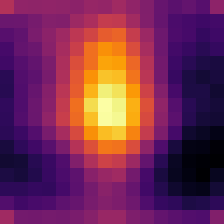
\includegraphics[width=\linewidth]{resources/231121_average_attn_location_reg2.png}
      \caption{reg$_2$}
   \end{subfigure}
   \hfill
  \begin{subfigure}[b]{0.15\textwidth}
      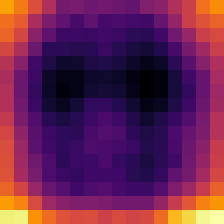
\includegraphics[width=\linewidth]{resources/231121_average_attn_location_reg3.png}
      \caption{reg$_3$}
   \end{subfigure}
   \hfill
  \begin{subfigure}[b]{0.15\textwidth}
      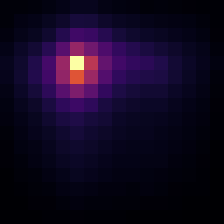
\includegraphics[width=\linewidth]{resources/231122_average_attmap_patch_1.png}
      \caption{patch}
   \end{subfigure}
   \hfill
  \caption{
  Average attention map of registers and \texttt{[CLS]} token. There is a variability observed, with register 3 of this model focusing more on border areas. We also include the average attention map of a patch for comparison. The patch has a much more focused average attention.
  }
  \label{fig:register_position_focus}
\end{figure}

In Fig. \ref{fig:register_position_focus} we display the positional focus for the class token and the 4 registers of a DINOv2+reg model.
We produce these plots by running the model on a random subset of ImageNet-22k, and averaging the attention maps for the corresponding tokens at the last layer. We note that ImageNet-22k contains mostly object-centric images rather than scenes, which explains why the average attention maps correspond to centered blobs.

We make several observations. First, the attention maps for registers can be different of each other; for example, register 3 tends to focus on border areas, while the other registers tend to focus on more centered areas. Register 2 tends to focus slightly more on the upper areas of images that others. This is consistent with Fig. \ref{fig:slot_attn}, where we show registers focusing on different large areas of the image, suggesting some level of specialization.

Second, by comparing the register maps to the \texttt{[CLS]} token map and to a patch token map, we observe that registers produce maps with a large support area, very similarly to the \texttt{[CLS]} token, and very different of a typical patch token which is more localized. As the \texttt{[CLS]} token is known to carry global information (as proven by the linear probing classification performance): this suggests that registers also carry global information.




\section{Masked autoencoders}
Masked Autoencoding \citep{he2021masked} is another common way of pretraining self-supervised models. We observe in Fig.~\ref{fig:mae_pca} that there are no artifacts in the maps produced by MAE: our hypothesis is that the absence of artifacts is due to the training procedure using only a local loss on the patch tokens, rather than an objective involving global aggregation of information. 
However, we also note that the performance of MAE models is very low for self-supervised representation learning (75\% linear probing performance on ImageNet classification for ViT-Large), preventing it from being used as is, and making fine-tuning a requirement.%


\begin{figure}[h]
  \centering
  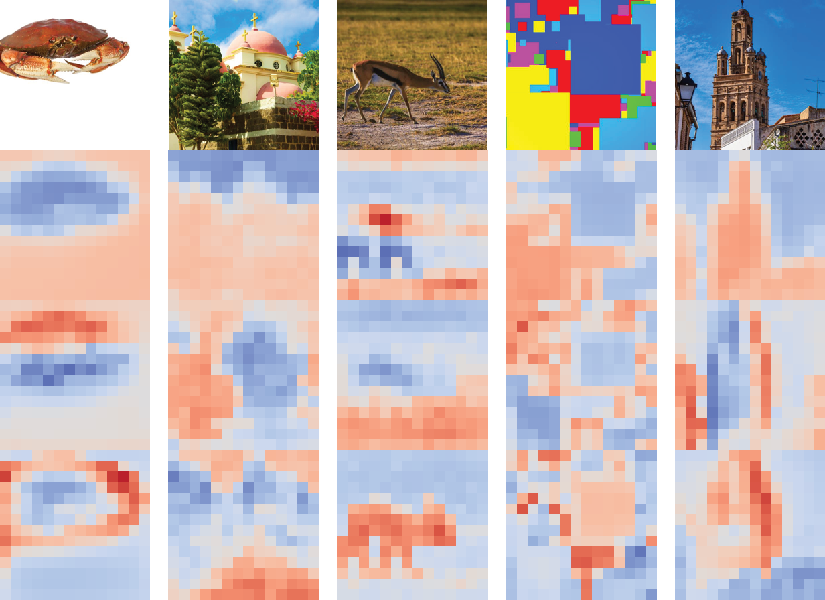
\includegraphics{resources/2023-11-22-mae.pdf}
  \caption{First three principal components of the output feature map of a ViT-Large Masked Autoencoder.}
  \label{fig:mae_pca}
\end{figure}

\section{Behavior per attention head}

In this section, we investigate whether the artifacts appear only on the attention maps for specific heads of the last vision transformer block, or for all of them.
We show in Fig.~\ref{fig:attmaps_per_head} the input image along with the attention maps for different heads. 
We observe that the artifacts appear for all attention heads, despite heads focusing on different areas of the object. 
We still observe that some heads focus more on artifacts than others.

\begin{figure}[h]
  \centering
  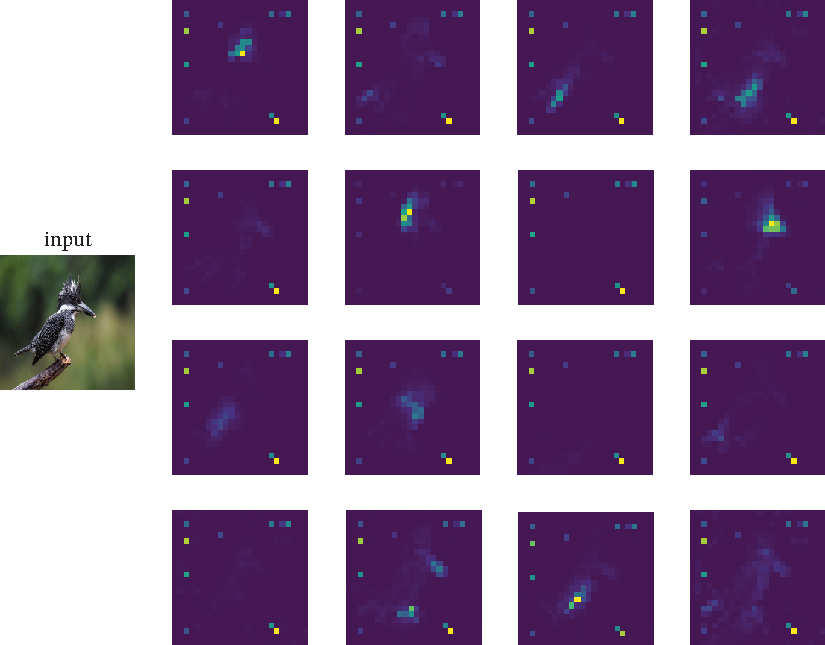
\includegraphics{resources/2023-11-22-heads.pdf}
  \caption{Attention maps of the \texttt{[CLS]} token to the patch tokens, shown here separately per attention head. We produce these maps with a DINOv2-L model trained without registers.}
  \label{fig:attmaps_per_head}
\end{figure}




\section{Variance on token information probing}
The results presented in table \ref{tab:logreg_weird_patches_image_classif} are obtained by taking a random patch token, either normal or outlier. However, the choice of this token adds a significant source of variance in the evaluation. For thoroughness, we report in table \ref{tab:logreg_weird_patches_image_classif_with_std} the standard deviation of the scores obtained relative to this choice.


\begin{table}[h]
    \centering
    
    \begin{tabular}{llllllll}
    \toprule
    dataset &                              Airc. &                               CF10 &                              CF100 &                                CUB &                             Cal101 &                               Cars &                                DTD \\
    token   &                                    &                                    &                                    &                                    &                                    &                                    &                                    \\
    \midrule
    normal  &  17.1\textcolor{gray}{\tiny{±0.5}} &  97.1\textcolor{gray}{\tiny{±0.1}} &  81.3\textcolor{gray}{\tiny{±0.3}} &  18.6\textcolor{gray}{\tiny{±0.6}} &  73.2\textcolor{gray}{\tiny{±1.3}} &  10.8\textcolor{gray}{\tiny{±0.3}} &  63.1\textcolor{gray}{\tiny{±0.8}} \\
    outlier &  79.1\textcolor{gray}{\tiny{±0.5}} &  99.3\textcolor{gray}{\tiny{±0.0}} &  93.7\textcolor{gray}{\tiny{±0.3}} &  84.9\textcolor{gray}{\tiny{±2.1}} &  97.6\textcolor{gray}{\tiny{±0.7}} &  85.2\textcolor{gray}{\tiny{±0.9}} &  84.9\textcolor{gray}{\tiny{±0.9}} \\
    \texttt{[CLS]} &                               87.3 &                               99.4 &                               94.5 &                               91.3 &                               96.9 &                               91.5 &                               85.2 \\
    \bottomrule
    \toprule
    dataset &                              Flow. &                               Food &                               IN1k &                               P205 &                               Pets &                                SUN &                                VOC \\
    token   &                                    &                                    &                                    &                                    &                                    &                                    &                                    \\
    \midrule
    normal  &  59.5\textcolor{gray}{\tiny{±1.2}} &  74.2\textcolor{gray}{\tiny{±0.3}} &  65.8\textcolor{gray}{\tiny{±0.1}} &  53.1\textcolor{gray}{\tiny{±0.3}} &  47.8\textcolor{gray}{\tiny{±0.5}} &  37.7\textcolor{gray}{\tiny{±0.3}} &  70.8\textcolor{gray}{\tiny{±0.5}} \\
    outlier &  99.6\textcolor{gray}{\tiny{±0.0}} &  93.5\textcolor{gray}{\tiny{±0.2}} &  69.0\textcolor{gray}{\tiny{±0.7}} &  55.1\textcolor{gray}{\tiny{±1.0}} &  94.1\textcolor{gray}{\tiny{±0.2}} &  78.5\textcolor{gray}{\tiny{±0.2}} &  89.7\textcolor{gray}{\tiny{±0.1}} \\
    \texttt{[CLS]} &                               99.7 &                               94.7 &                               86.0 &                               66.4 &                               96.9 &                               78.6 &                               89.1 \\
    \bottomrule
    \end{tabular}
    \caption{Image classification via linear probing on normal and outlier patch tokens. As we select the patch tokens randomly among the set of eligible tokens, this adds a source of variability. We report the standard deviation of this variability in grey along with the scores. This table is a detailed view of table \ref{tab:logreg_weird_patches_image_classif}.}
    \label{tab:logreg_weird_patches_image_classif_with_std}
\end{table}


\section{Qualitative Results}
\label{sec:appendix_qualitative}
We trained three popular models: DeiT-III, OpenCLIP, DINOv2 with and without the introduction of register tokens.
We observe in Fig. \ref{fig:supmat_pagefig_attmaps_beforeafter} the attention maps in the last layer of the Vision Transformer, for all three cases.
We see that our approach provides much cleaner attention maps, with considerably fewer artifacts, explaining the improvement on the downstream object discovery task mentioned in Sec. \ref{sec:obj_discovery}.
The feature maps are also visibly improved, as shown in Fig. \ref{fig:supmat_pagefig_pca_beforeafter}.
Finally, we also show the norm of the patch tokens in Fig. \ref{fig:supmat_pagefig_norms_beforeafter}, and confirm that in all three models, artifact patches correspond to norm outliers.


\newpage



\begin{figure}[h]
    \centering
    {\footnotesize
    \setlength{\tabcolsep}{2.5pt} %
    \renewcommand{\arraystretch}{0.4} %
    \begin{tabular}{c @{\hspace{5mm}} c@{ }c @{ } c@{\hspace{5mm}}c @{ } c@{ }c }
        \vspace{0.2em}
        & \multicolumn{3}{c}{Without registers} & \multicolumn{3}{c}{With registers} \\
        Input & DeiT-III & OpenCLIP & DINOv2 & DeiT-III & OpenCLIP & DINOv2 \\
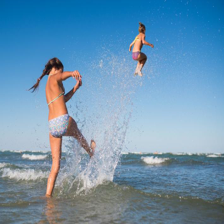
\includegraphics[width=0.13\textwidth]{resources/230914_1202_fig2_vizs_various_models/109_orig.png} &
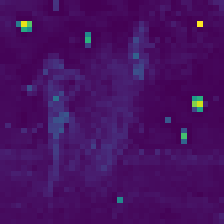
\includegraphics[width=0.13\textwidth]{resources/230915_1613_fig1_attmaps_before_after/deit3_0reg_109_lastattmap.png} &
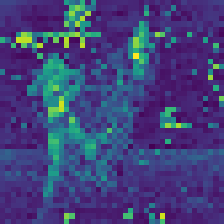
\includegraphics[width=0.13\textwidth]{resources/230915_1613_fig1_attmaps_before_after/clip_0reg_109_lastattmap.png} &
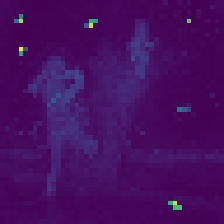
\includegraphics[width=0.13\textwidth]{resources/230915_1613_fig1_attmaps_before_after/dinov2_0reg_109_lastattmap.png} &
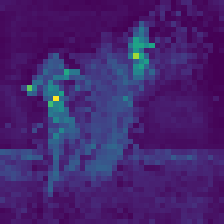
\includegraphics[width=0.13\textwidth]{resources/230915_1613_fig1_attmaps_before_after/deit3_4reg_109_lastattmap.png} &
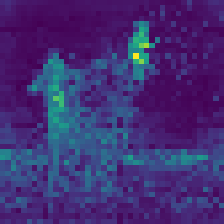
\includegraphics[width=0.13\textwidth]{resources/230915_1613_fig1_attmaps_before_after/clip_4reg_109_lastattmap.png} &
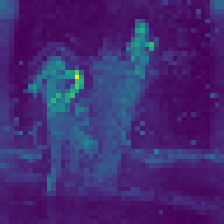
\includegraphics[width=0.13\textwidth]{resources/230915_1613_fig1_attmaps_before_after/dinov2_4reg_109_lastattmap.png} \\
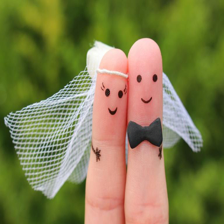
\includegraphics[width=0.13\textwidth]{resources/230914_1202_fig2_vizs_various_models/226_orig.png} &
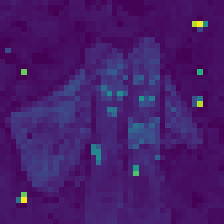
\includegraphics[width=0.13\textwidth]{resources/230915_1613_fig1_attmaps_before_after/deit3_0reg_226_lastattmap.png} &
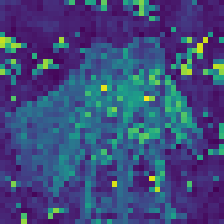
\includegraphics[width=0.13\textwidth]{resources/230915_1613_fig1_attmaps_before_after/clip_0reg_226_lastattmap.png} &
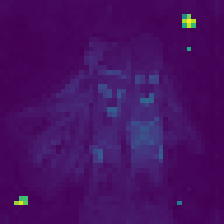
\includegraphics[width=0.13\textwidth]{resources/230915_1613_fig1_attmaps_before_after/dinov2_0reg_226_lastattmap.png} &
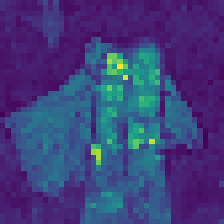
\includegraphics[width=0.13\textwidth]{resources/230915_1613_fig1_attmaps_before_after/deit3_4reg_226_lastattmap.png} &
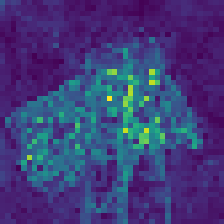
\includegraphics[width=0.13\textwidth]{resources/230915_1613_fig1_attmaps_before_after/clip_4reg_226_lastattmap.png} &
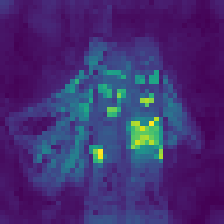
\includegraphics[width=0.13\textwidth]{resources/230915_1613_fig1_attmaps_before_after/dinov2_4reg_226_lastattmap.png} \\
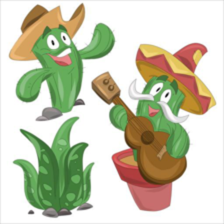
\includegraphics[width=0.13\textwidth]{resources/230916_1943_fig1_attmaps_before_after_100cc/900_orig.png} &
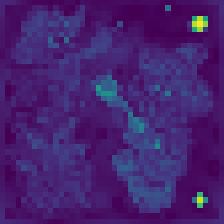
\includegraphics[width=0.13\textwidth]{resources/230916_1943_fig1_attmaps_before_after_100cc/deit3_0reg_900_lastattmap.png} &
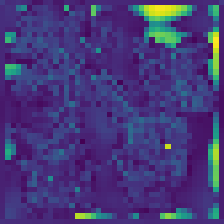
\includegraphics[width=0.13\textwidth]{resources/230916_1943_fig1_attmaps_before_after_100cc/clip_0reg_900_lastattmap.png} &
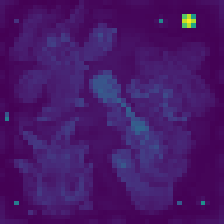
\includegraphics[width=0.13\textwidth]{resources/230916_1943_fig1_attmaps_before_after_100cc/dinov2_0reg_900_lastattmap.png} &
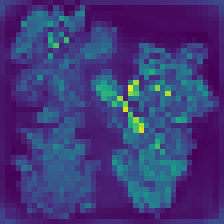
\includegraphics[width=0.13\textwidth]{resources/230916_1943_fig1_attmaps_before_after_100cc/deit3_4reg_900_lastattmap.png} &
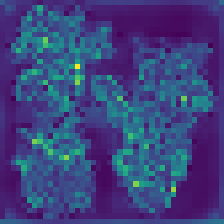
\includegraphics[width=0.13\textwidth]{resources/230916_1943_fig1_attmaps_before_after_100cc/clip_4reg_900_lastattmap.png} &
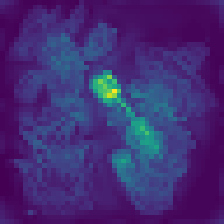
\includegraphics[width=0.13\textwidth]{resources/230916_1943_fig1_attmaps_before_after_100cc/dinov2_4reg_900_lastattmap.png} \\
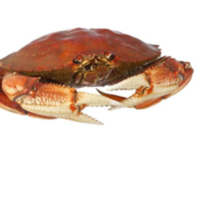
\includegraphics[width=0.13\textwidth]{resources/230916_1943_fig1_attmaps_before_after_100cc/218_orig.png} &
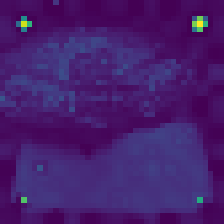
\includegraphics[width=0.13\textwidth]{resources/230916_1943_fig1_attmaps_before_after_100cc/deit3_0reg_218_lastattmap.png} &
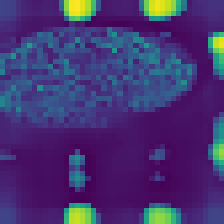
\includegraphics[width=0.13\textwidth]{resources/230916_1943_fig1_attmaps_before_after_100cc/clip_0reg_218_lastattmap.png} &
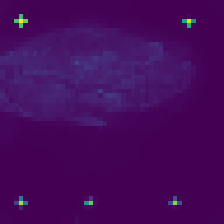
\includegraphics[width=0.13\textwidth]{resources/230916_1943_fig1_attmaps_before_after_100cc/dinov2_0reg_218_lastattmap.png} &
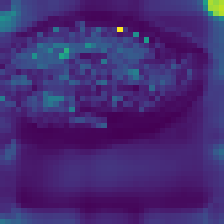
\includegraphics[width=0.13\textwidth]{resources/230916_1943_fig1_attmaps_before_after_100cc/deit3_4reg_218_lastattmap.png} &
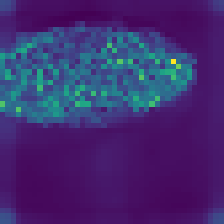
\includegraphics[width=0.13\textwidth]{resources/230916_1943_fig1_attmaps_before_after_100cc/clip_4reg_218_lastattmap.png} &
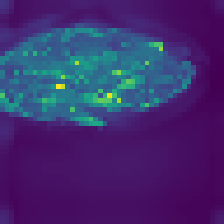
\includegraphics[width=0.13\textwidth]{resources/230916_1943_fig1_attmaps_before_after_100cc/dinov2_4reg_218_lastattmap.png} \\

\includegraphics[width=0.13\textwidth]{resources/230916_1943_fig1_attmaps_before_after_100cc/219_orig.png} &
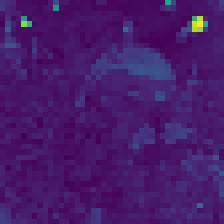
\includegraphics[width=0.13\textwidth]{resources/230916_1943_fig1_attmaps_before_after_100cc/deit3_0reg_219_lastattmap.png} &
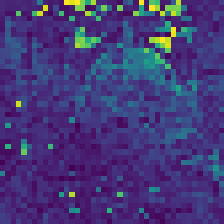
\includegraphics[width=0.13\textwidth]{resources/230916_1943_fig1_attmaps_before_after_100cc/clip_0reg_219_lastattmap.png} &
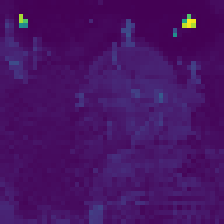
\includegraphics[width=0.13\textwidth]{resources/230916_1943_fig1_attmaps_before_after_100cc/dinov2_0reg_219_lastattmap.png} &
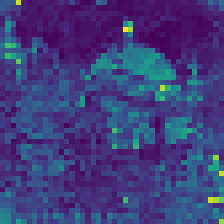
\includegraphics[width=0.13\textwidth]{resources/230916_1943_fig1_attmaps_before_after_100cc/deit3_4reg_219_lastattmap.png} &
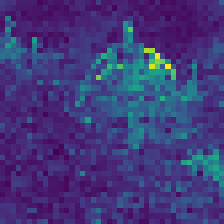
\includegraphics[width=0.13\textwidth]{resources/230916_1943_fig1_attmaps_before_after_100cc/clip_4reg_219_lastattmap.png} &
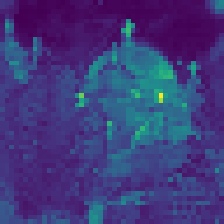
\includegraphics[width=0.13\textwidth]{resources/230916_1943_fig1_attmaps_before_after_100cc/dinov2_4reg_219_lastattmap.png} \\
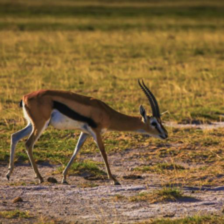
\includegraphics[width=0.13\textwidth]{resources/230916_1943_fig1_attmaps_before_after_100cc/242_orig.png} &
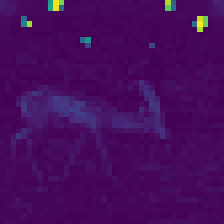
\includegraphics[width=0.13\textwidth]{resources/230916_1943_fig1_attmaps_before_after_100cc/deit3_0reg_242_lastattmap.png} &
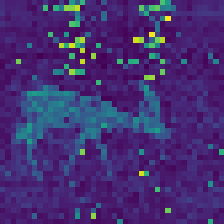
\includegraphics[width=0.13\textwidth]{resources/230916_1943_fig1_attmaps_before_after_100cc/clip_0reg_242_lastattmap.png} &
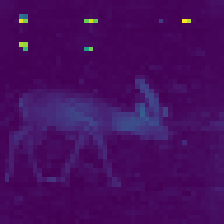
\includegraphics[width=0.13\textwidth]{resources/230916_1943_fig1_attmaps_before_after_100cc/dinov2_0reg_242_lastattmap.png} &
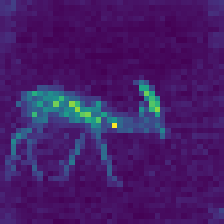
\includegraphics[width=0.13\textwidth]{resources/230916_1943_fig1_attmaps_before_after_100cc/deit3_4reg_242_lastattmap.png} &
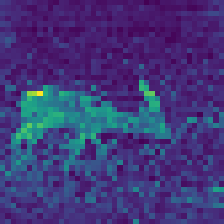
\includegraphics[width=0.13\textwidth]{resources/230916_1943_fig1_attmaps_before_after_100cc/clip_4reg_242_lastattmap.png} &
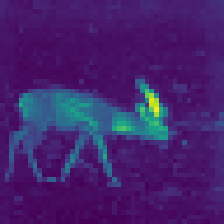
\includegraphics[width=0.13\textwidth]{resources/230916_1943_fig1_attmaps_before_after_100cc/dinov2_4reg_242_lastattmap.png} \\

\includegraphics[width=0.13\textwidth]{resources/230916_1943_fig1_attmaps_before_after_100cc/285_orig.png} &
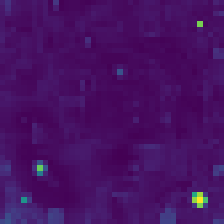
\includegraphics[width=0.13\textwidth]{resources/230916_1943_fig1_attmaps_before_after_100cc/deit3_0reg_285_lastattmap.png} &
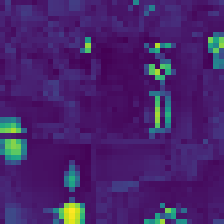
\includegraphics[width=0.13\textwidth]{resources/230916_1943_fig1_attmaps_before_after_100cc/clip_0reg_285_lastattmap.png} &
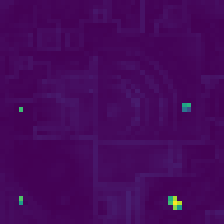
\includegraphics[width=0.13\textwidth]{resources/230916_1943_fig1_attmaps_before_after_100cc/dinov2_0reg_285_lastattmap.png} &
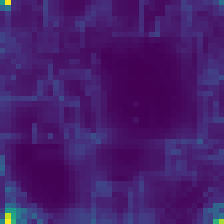
\includegraphics[width=0.13\textwidth]{resources/230916_1943_fig1_attmaps_before_after_100cc/deit3_4reg_285_lastattmap.png} &
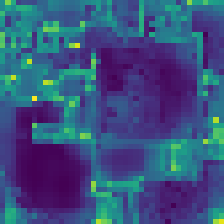
\includegraphics[width=0.13\textwidth]{resources/230916_1943_fig1_attmaps_before_after_100cc/clip_4reg_285_lastattmap.png} &
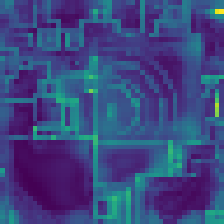
\includegraphics[width=0.13\textwidth]{resources/230916_1943_fig1_attmaps_before_after_100cc/dinov2_4reg_285_lastattmap.png} \\
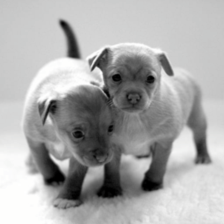
\includegraphics[width=0.13\textwidth]{resources/230916_1943_fig1_attmaps_before_after_100cc/405_orig.png} &
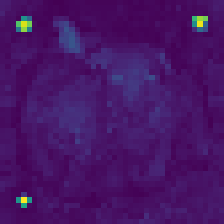
\includegraphics[width=0.13\textwidth]{resources/230916_1943_fig1_attmaps_before_after_100cc/deit3_0reg_405_lastattmap.png} &
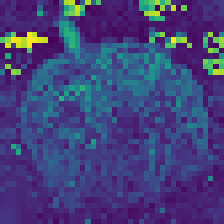
\includegraphics[width=0.13\textwidth]{resources/230916_1943_fig1_attmaps_before_after_100cc/clip_0reg_405_lastattmap.png} &
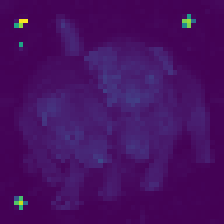
\includegraphics[width=0.13\textwidth]{resources/230916_1943_fig1_attmaps_before_after_100cc/dinov2_0reg_405_lastattmap.png} &
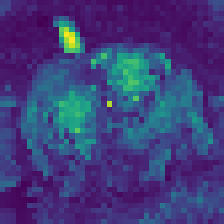
\includegraphics[width=0.13\textwidth]{resources/230916_1943_fig1_attmaps_before_after_100cc/deit3_4reg_405_lastattmap.png} &
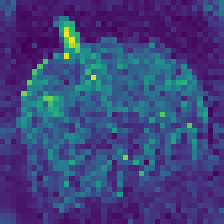
\includegraphics[width=0.13\textwidth]{resources/230916_1943_fig1_attmaps_before_after_100cc/clip_4reg_405_lastattmap.png} &
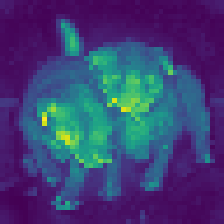
\includegraphics[width=0.13\textwidth]{resources/230916_1943_fig1_attmaps_before_after_100cc/dinov2_4reg_405_lastattmap.png} \\
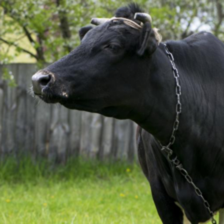
\includegraphics[width=0.13\textwidth]{resources/230916_1943_fig1_attmaps_before_after_100cc/512_orig.png} &
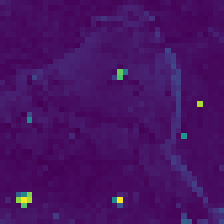
\includegraphics[width=0.13\textwidth]{resources/230916_1943_fig1_attmaps_before_after_100cc/deit3_0reg_512_lastattmap.png} &
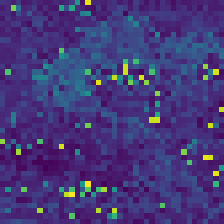
\includegraphics[width=0.13\textwidth]{resources/230916_1943_fig1_attmaps_before_after_100cc/clip_0reg_512_lastattmap.png} &
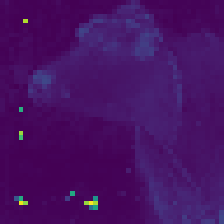
\includegraphics[width=0.13\textwidth]{resources/230916_1943_fig1_attmaps_before_after_100cc/dinov2_0reg_512_lastattmap.png} &
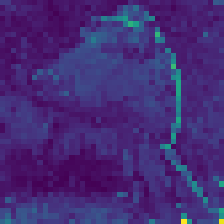
\includegraphics[width=0.13\textwidth]{resources/230916_1943_fig1_attmaps_before_after_100cc/deit3_4reg_512_lastattmap.png} &
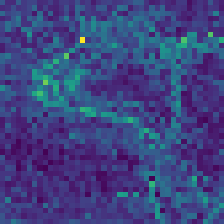
\includegraphics[width=0.13\textwidth]{resources/230916_1943_fig1_attmaps_before_after_100cc/clip_4reg_512_lastattmap.png} &
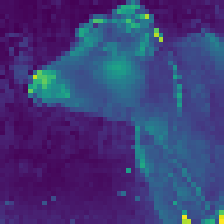
\includegraphics[width=0.13\textwidth]{resources/230916_1943_fig1_attmaps_before_after_100cc/dinov2_4reg_512_lastattmap.png} \\
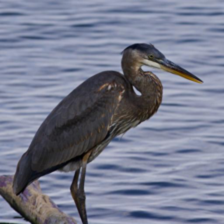
\includegraphics[width=0.13\textwidth]{resources/230916_1943_fig1_attmaps_before_after_100cc/513_orig.png} &
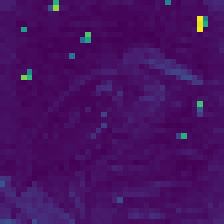
\includegraphics[width=0.13\textwidth]{resources/230916_1943_fig1_attmaps_before_after_100cc/deit3_0reg_513_lastattmap.png} &
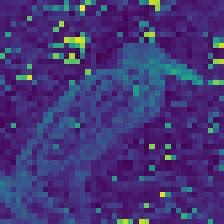
\includegraphics[width=0.13\textwidth]{resources/230916_1943_fig1_attmaps_before_after_100cc/clip_0reg_513_lastattmap.png} &
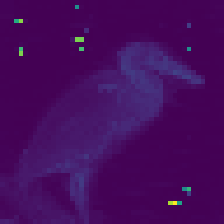
\includegraphics[width=0.13\textwidth]{resources/230916_1943_fig1_attmaps_before_after_100cc/dinov2_0reg_513_lastattmap.png} &
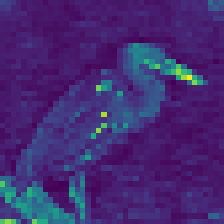
\includegraphics[width=0.13\textwidth]{resources/230916_1943_fig1_attmaps_before_after_100cc/deit3_4reg_513_lastattmap.png} &
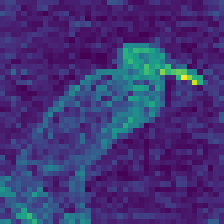
\includegraphics[width=0.13\textwidth]{resources/230916_1943_fig1_attmaps_before_after_100cc/clip_4reg_513_lastattmap.png} &
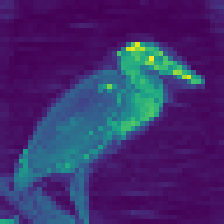
\includegraphics[width=0.13\textwidth]{resources/230916_1943_fig1_attmaps_before_after_100cc/dinov2_4reg_513_lastattmap.png} \\
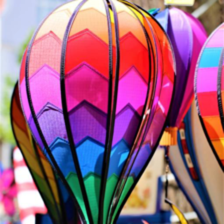
\includegraphics[width=0.13\textwidth]{resources/230916_1943_fig1_attmaps_before_after_100cc/532_orig.png} &
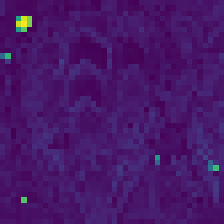
\includegraphics[width=0.13\textwidth]{resources/230916_1943_fig1_attmaps_before_after_100cc/deit3_0reg_532_lastattmap.png} &
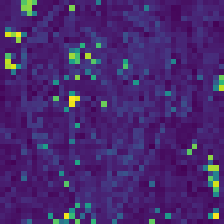
\includegraphics[width=0.13\textwidth]{resources/230916_1943_fig1_attmaps_before_after_100cc/clip_0reg_532_lastattmap.png} &

\includegraphics[width=0.13\textwidth]{resources/230916_1943_fig1_attmaps_before_after_100cc/dinov2_0reg_532_lastattmap.png} &
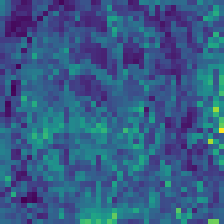
\includegraphics[width=0.13\textwidth]{resources/230916_1943_fig1_attmaps_before_after_100cc/deit3_4reg_532_lastattmap.png} &
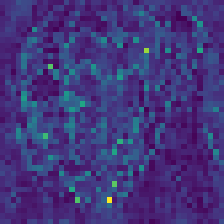
\includegraphics[width=0.13\textwidth]{resources/230916_1943_fig1_attmaps_before_after_100cc/clip_4reg_532_lastattmap.png} &
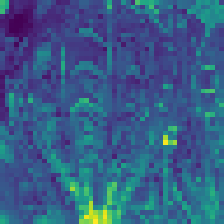
\includegraphics[width=0.13\textwidth]{resources/230916_1943_fig1_attmaps_before_after_100cc/dinov2_4reg_532_lastattmap.png} \\

    \end{tabular}
    }
    \caption{Attention maps of models trained without and with registers on various images.}
    \label{fig:supmat_pagefig_attmaps_beforeafter}
  \end{figure}



\begin{figure}[h]
    \centering
    {\footnotesize
    \setlength{\tabcolsep}{2.5pt} %
    \renewcommand{\arraystretch}{0.4} %
    \begin{tabular}{c @{\hspace{5mm}} c@{ }c @{ } c@{\hspace{5mm}}c @{ } c@{ }c }
        \vspace{0.2em}
        & \multicolumn{3}{c}{Without registers} & \multicolumn{3}{c}{With registers} \\
        Input & DeiT-III & OpenCLIP & DINOv2 & DeiT-III & OpenCLIP & DINOv2 \\
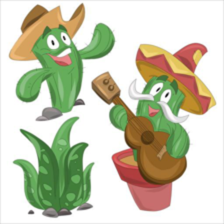
\includegraphics[width=0.13\textwidth]{resources/230916_1943_fig1_attmaps_before_after_100cc/900_orig.png} &
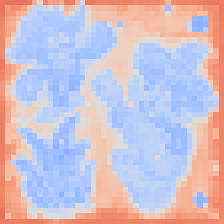
\includegraphics[width=0.13\textwidth]{resources/230916_1943_fig1_attmaps_before_after_100cc/deit3_0reg_900_pca_0.png} &
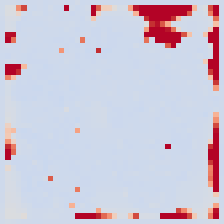
\includegraphics[width=0.13\textwidth]{resources/230916_1943_fig1_attmaps_before_after_100cc/clip_0reg_900_pca_0.png} &
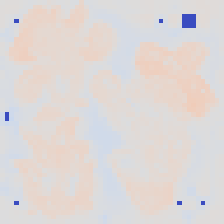
\includegraphics[width=0.13\textwidth]{resources/230916_1943_fig1_attmaps_before_after_100cc/dinov2_0reg_900_pca_0.png} &
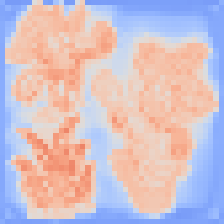
\includegraphics[width=0.13\textwidth]{resources/230916_1943_fig1_attmaps_before_after_100cc/deit3_4reg_900_pca_0.png} &
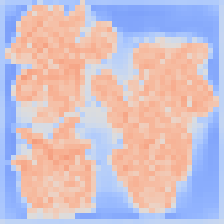
\includegraphics[width=0.13\textwidth]{resources/230916_1943_fig1_attmaps_before_after_100cc/clip_4reg_900_pca_0.png} &
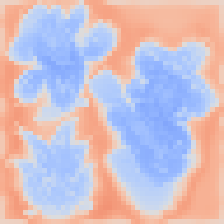
\includegraphics[width=0.13\textwidth]{resources/230916_1943_fig1_attmaps_before_after_100cc/dinov2_4reg_900_pca_0.png} \\
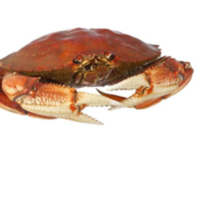
\includegraphics[width=0.13\textwidth]{resources/230916_1943_fig1_attmaps_before_after_100cc/218_orig.png} &
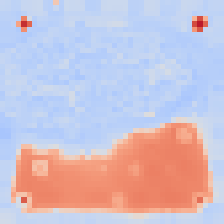
\includegraphics[width=0.13\textwidth]{resources/230916_1943_fig1_attmaps_before_after_100cc/deit3_0reg_218_pca_0.png} &
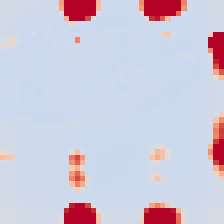
\includegraphics[width=0.13\textwidth]{resources/230916_1943_fig1_attmaps_before_after_100cc/clip_0reg_218_pca_0.png} &
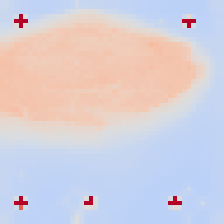
\includegraphics[width=0.13\textwidth]{resources/230916_1943_fig1_attmaps_before_after_100cc/dinov2_0reg_218_pca_0.png} &

\includegraphics[width=0.13\textwidth]{resources/230916_1943_fig1_attmaps_before_after_100cc/deit3_4reg_218_pca_0.png} &

\includegraphics[width=0.13\textwidth]{resources/230916_1943_fig1_attmaps_before_after_100cc/clip_4reg_218_pca_0.png} &

\includegraphics[width=0.13\textwidth]{resources/230916_1943_fig1_attmaps_before_after_100cc/dinov2_4reg_218_pca_0.png} \\

\includegraphics[width=0.13\textwidth]{resources/230916_1943_fig1_attmaps_before_after_100cc/219_orig.png} &

\includegraphics[width=0.13\textwidth]{resources/230916_1943_fig1_attmaps_before_after_100cc/deit3_0reg_219_pca_0.png} &
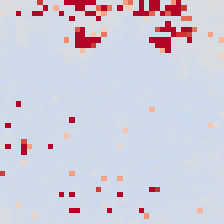
\includegraphics[width=0.13\textwidth]{resources/230916_1943_fig1_attmaps_before_after_100cc/clip_0reg_219_pca_0.png} &
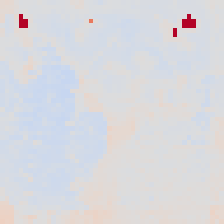
\includegraphics[width=0.13\textwidth]{resources/230916_1943_fig1_attmaps_before_after_100cc/dinov2_0reg_219_pca_0.png} &

\includegraphics[width=0.13\textwidth]{resources/230916_1943_fig1_attmaps_before_after_100cc/deit3_4reg_219_pca_0.png} &

\includegraphics[width=0.13\textwidth]{resources/230916_1943_fig1_attmaps_before_after_100cc/clip_4reg_219_pca_0.png} &
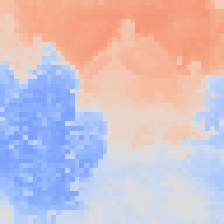
\includegraphics[width=0.13\textwidth]{resources/230916_1943_fig1_attmaps_before_after_100cc/dinov2_4reg_219_pca_0.png} \\
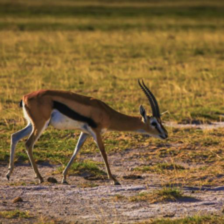
\includegraphics[width=0.13\textwidth]{resources/230916_1943_fig1_attmaps_before_after_100cc/242_orig.png} &
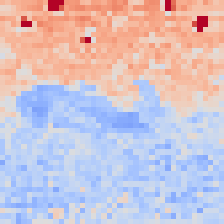
\includegraphics[width=0.13\textwidth]{resources/230916_1943_fig1_attmaps_before_after_100cc/deit3_0reg_242_pca_0.png} &

\includegraphics[width=0.13\textwidth]{resources/230916_1943_fig1_attmaps_before_after_100cc/clip_0reg_242_pca_0.png} &
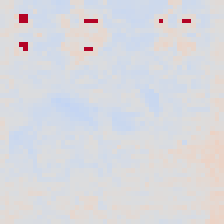
\includegraphics[width=0.13\textwidth]{resources/230916_1943_fig1_attmaps_before_after_100cc/dinov2_0reg_242_pca_0.png} &
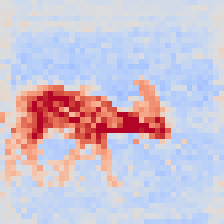
\includegraphics[width=0.13\textwidth]{resources/230916_1943_fig1_attmaps_before_after_100cc/deit3_4reg_242_pca_0.png} &
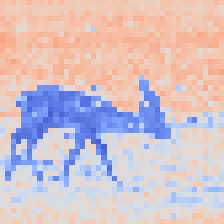
\includegraphics[width=0.13\textwidth]{resources/230916_1943_fig1_attmaps_before_after_100cc/clip_4reg_242_pca_0.png} &
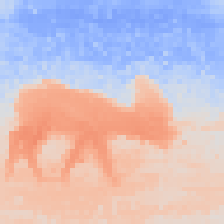
\includegraphics[width=0.13\textwidth]{resources/230916_1943_fig1_attmaps_before_after_100cc/dinov2_4reg_242_pca_0.png} \\

\includegraphics[width=0.13\textwidth]{resources/230916_1943_fig1_attmaps_before_after_100cc/285_orig.png} &
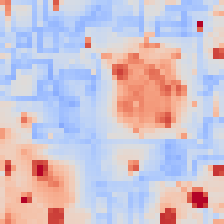
\includegraphics[width=0.13\textwidth]{resources/230916_1943_fig1_attmaps_before_after_100cc/deit3_0reg_285_pca_0.png} &
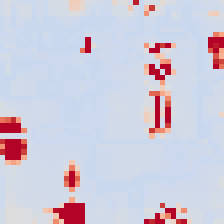
\includegraphics[width=0.13\textwidth]{resources/230916_1943_fig1_attmaps_before_after_100cc/clip_0reg_285_pca_0.png} &

\includegraphics[width=0.13\textwidth]{resources/230916_1943_fig1_attmaps_before_after_100cc/dinov2_0reg_285_pca_0.png} &
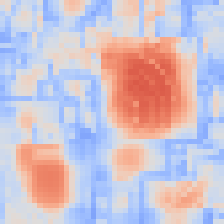
\includegraphics[width=0.13\textwidth]{resources/230916_1943_fig1_attmaps_before_after_100cc/deit3_4reg_285_pca_0.png} &
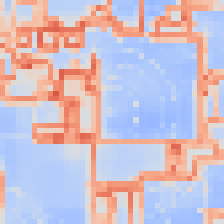
\includegraphics[width=0.13\textwidth]{resources/230916_1943_fig1_attmaps_before_after_100cc/clip_4reg_285_pca_0.png} &
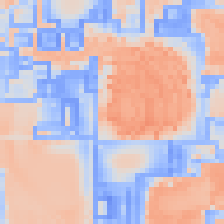
\includegraphics[width=0.13\textwidth]{resources/230916_1943_fig1_attmaps_before_after_100cc/dinov2_4reg_285_pca_0.png} \\
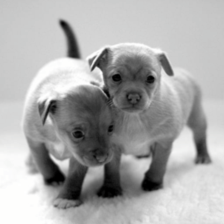
\includegraphics[width=0.13\textwidth]{resources/230916_1943_fig1_attmaps_before_after_100cc/405_orig.png} &
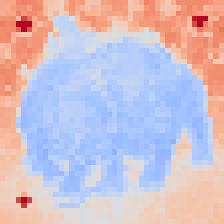
\includegraphics[width=0.13\textwidth]{resources/230916_1943_fig1_attmaps_before_after_100cc/deit3_0reg_405_pca_0.png} &

\includegraphics[width=0.13\textwidth]{resources/230916_1943_fig1_attmaps_before_after_100cc/clip_0reg_405_pca_0.png} &

\includegraphics[width=0.13\textwidth]{resources/230916_1943_fig1_attmaps_before_after_100cc/dinov2_0reg_405_pca_0.png} &

\includegraphics[width=0.13\textwidth]{resources/230916_1943_fig1_attmaps_before_after_100cc/deit3_4reg_405_pca_0.png} &

\includegraphics[width=0.13\textwidth]{resources/230916_1943_fig1_attmaps_before_after_100cc/clip_4reg_405_pca_0.png} &

\includegraphics[width=0.13\textwidth]{resources/230916_1943_fig1_attmaps_before_after_100cc/dinov2_4reg_405_pca_0.png} \\
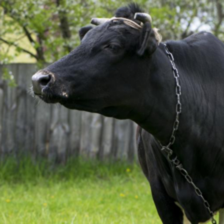
\includegraphics[width=0.13\textwidth]{resources/230916_1943_fig1_attmaps_before_after_100cc/512_orig.png} &
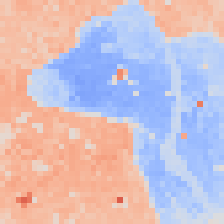
\includegraphics[width=0.13\textwidth]{resources/230916_1943_fig1_attmaps_before_after_100cc/deit3_0reg_512_pca_0.png} &
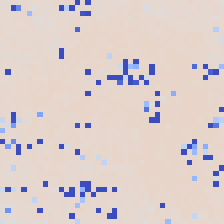
\includegraphics[width=0.13\textwidth]{resources/230916_1943_fig1_attmaps_before_after_100cc/clip_0reg_512_pca_0.png} &
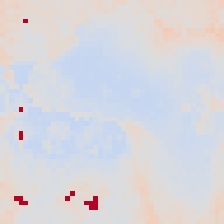
\includegraphics[width=0.13\textwidth]{resources/230916_1943_fig1_attmaps_before_after_100cc/dinov2_0reg_512_pca_0.png} &

\includegraphics[width=0.13\textwidth]{resources/230916_1943_fig1_attmaps_before_after_100cc/deit3_4reg_512_pca_0.png} &

\includegraphics[width=0.13\textwidth]{resources/230916_1943_fig1_attmaps_before_after_100cc/clip_4reg_512_pca_0.png} &

\includegraphics[width=0.13\textwidth]{resources/230916_1943_fig1_attmaps_before_after_100cc/dinov2_4reg_512_pca_0.png} \\
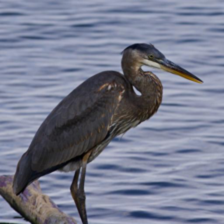
\includegraphics[width=0.13\textwidth]{resources/230916_1943_fig1_attmaps_before_after_100cc/513_orig.png} &
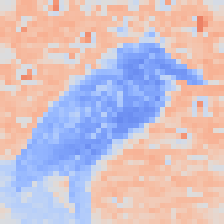
\includegraphics[width=0.13\textwidth]{resources/230916_1943_fig1_attmaps_before_after_100cc/deit3_0reg_513_pca_0.png} &

\includegraphics[width=0.13\textwidth]{resources/230916_1943_fig1_attmaps_before_after_100cc/clip_0reg_513_pca_0.png} &

\includegraphics[width=0.13\textwidth]{resources/230916_1943_fig1_attmaps_before_after_100cc/dinov2_0reg_513_pca_0.png} &

\includegraphics[width=0.13\textwidth]{resources/230916_1943_fig1_attmaps_before_after_100cc/deit3_4reg_513_pca_0.png} &

\includegraphics[width=0.13\textwidth]{resources/230916_1943_fig1_attmaps_before_after_100cc/clip_4reg_513_pca_0.png} &
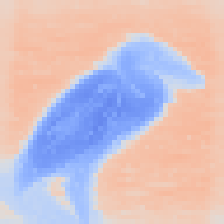
\includegraphics[width=0.13\textwidth]{resources/230916_1943_fig1_attmaps_before_after_100cc/dinov2_4reg_513_pca_0.png} \\
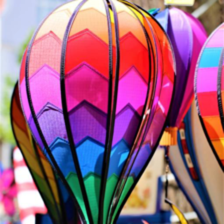
\includegraphics[width=0.13\textwidth]{resources/230916_1943_fig1_attmaps_before_after_100cc/532_orig.png} &

\includegraphics[width=0.13\textwidth]{resources/230916_1943_fig1_attmaps_before_after_100cc/deit3_0reg_532_pca_0.png} &
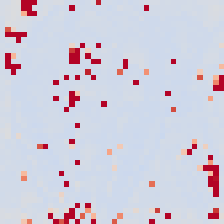
\includegraphics[width=0.13\textwidth]{resources/230916_1943_fig1_attmaps_before_after_100cc/clip_0reg_532_pca_0.png} &
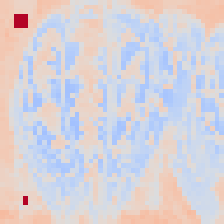
\includegraphics[width=0.13\textwidth]{resources/230916_1943_fig1_attmaps_before_after_100cc/dinov2_0reg_532_pca_0.png} &

\includegraphics[width=0.13\textwidth]{resources/230916_1943_fig1_attmaps_before_after_100cc/deit3_4reg_532_pca_0.png} &

\includegraphics[width=0.13\textwidth]{resources/230916_1943_fig1_attmaps_before_after_100cc/clip_4reg_532_pca_0.png} &
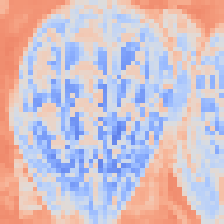
\includegraphics[width=0.13\textwidth]{resources/230916_1943_fig1_attmaps_before_after_100cc/dinov2_4reg_532_pca_0.png} \\
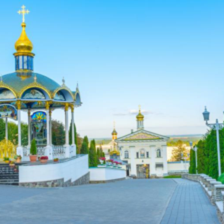
\includegraphics[width=0.13\textwidth]{resources/230916_1943_fig1_attmaps_before_after_100cc/552_orig.png} &
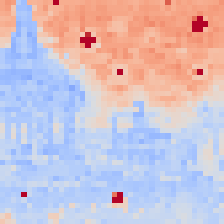
\includegraphics[width=0.13\textwidth]{resources/230916_1943_fig1_attmaps_before_after_100cc/deit3_0reg_552_pca_0.png} &

\includegraphics[width=0.13\textwidth]{resources/230916_1943_fig1_attmaps_before_after_100cc/clip_0reg_552_pca_0.png} &

\includegraphics[width=0.13\textwidth]{resources/230916_1943_fig1_attmaps_before_after_100cc/dinov2_0reg_552_pca_0.png} &

\includegraphics[width=0.13\textwidth]{resources/230916_1943_fig1_attmaps_before_after_100cc/deit3_4reg_552_pca_0.png} &

\includegraphics[width=0.13\textwidth]{resources/230916_1943_fig1_attmaps_before_after_100cc/clip_4reg_552_pca_0.png} &

\includegraphics[width=0.13\textwidth]{resources/230916_1943_fig1_attmaps_before_after_100cc/dinov2_4reg_552_pca_0.png} \\

\includegraphics[width=0.13\textwidth]{resources/230916_1943_fig1_attmaps_before_after_100cc/553_orig.png} &
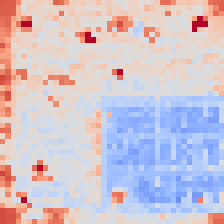
\includegraphics[width=0.13\textwidth]{resources/230916_1943_fig1_attmaps_before_after_100cc/deit3_0reg_553_pca_0.png} &

\includegraphics[width=0.13\textwidth]{resources/230916_1943_fig1_attmaps_before_after_100cc/clip_0reg_553_pca_0.png} &
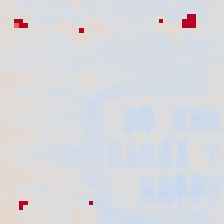
\includegraphics[width=0.13\textwidth]{resources/230916_1943_fig1_attmaps_before_after_100cc/dinov2_0reg_553_pca_0.png} &

\includegraphics[width=0.13\textwidth]{resources/230916_1943_fig1_attmaps_before_after_100cc/deit3_4reg_553_pca_0.png} &

\includegraphics[width=0.13\textwidth]{resources/230916_1943_fig1_attmaps_before_after_100cc/clip_4reg_553_pca_0.png} &

\includegraphics[width=0.13\textwidth]{resources/230916_1943_fig1_attmaps_before_after_100cc/dinov2_4reg_553_pca_0.png} \\

    \end{tabular}
    }
    \caption{
        First principal component of the feature maps output by models trained without and with registers on various images.
        The components are whitened and the colormap covers the range $[-3\sigma, +3\sigma]$.
        }
    \label{fig:supmat_pagefig_pca_beforeafter}
  \end{figure}

  




\begin{figure}[h]
    \centering
    {\footnotesize
    \setlength{\tabcolsep}{2.5pt} %
    \renewcommand{\arraystretch}{0.4} %
    \begin{tabular}{c @{\hspace{5mm}} c@{ }c @{ } c@{\hspace{5mm}}c @{ } c@{ }c }
        \vspace{0.2em}
        & \multicolumn{3}{c}{Without registers} & \multicolumn{3}{c}{With registers} \\
        Input & DeiT-III & OpenCLIP & DINOv2 & DeiT-III & OpenCLIP & DINOv2 \\
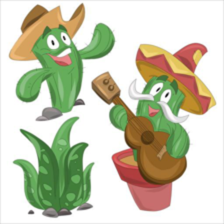
\includegraphics[width=0.13\textwidth]{resources/230916_1943_fig1_attmaps_before_after_100cc/900_orig.png} &
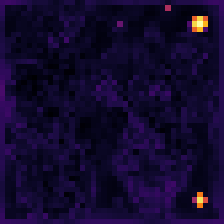
\includegraphics[width=0.13\textwidth]{resources/230916_1943_fig1_attmaps_before_after_100cc/deit3_0reg_900_norms.png} &
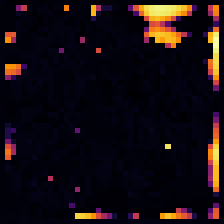
\includegraphics[width=0.13\textwidth]{resources/230916_1943_fig1_attmaps_before_after_100cc/clip_0reg_900_norms.png} &
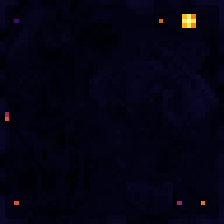
\includegraphics[width=0.13\textwidth]{resources/230916_1943_fig1_attmaps_before_after_100cc/dinov2_0reg_900_norms.png} &
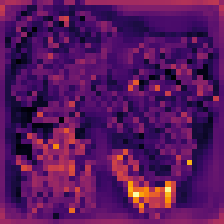
\includegraphics[width=0.13\textwidth]{resources/230916_1943_fig1_attmaps_before_after_100cc/deit3_4reg_900_norms.png} &
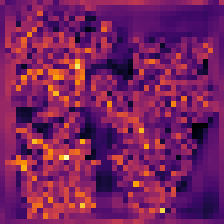
\includegraphics[width=0.13\textwidth]{resources/230916_1943_fig1_attmaps_before_after_100cc/clip_4reg_900_norms.png} &
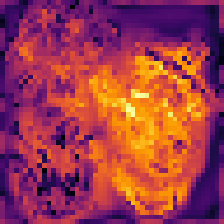
\includegraphics[width=0.13\textwidth]{resources/230916_1943_fig1_attmaps_before_after_100cc/dinov2_4reg_900_norms.png} \\
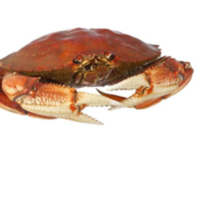
\includegraphics[width=0.13\textwidth]{resources/230916_1943_fig1_attmaps_before_after_100cc/218_orig.png} &
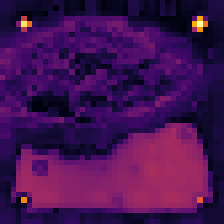
\includegraphics[width=0.13\textwidth]{resources/230916_1943_fig1_attmaps_before_after_100cc/deit3_0reg_218_norms.png} &
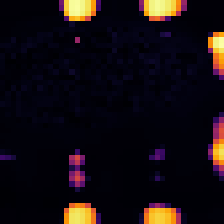
\includegraphics[width=0.13\textwidth]{resources/230916_1943_fig1_attmaps_before_after_100cc/clip_0reg_218_norms.png} &
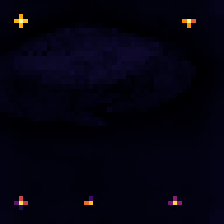
\includegraphics[width=0.13\textwidth]{resources/230916_1943_fig1_attmaps_before_after_100cc/dinov2_0reg_218_norms.png} &
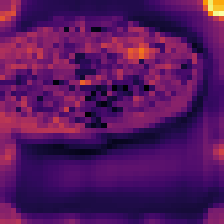
\includegraphics[width=0.13\textwidth]{resources/230916_1943_fig1_attmaps_before_after_100cc/deit3_4reg_218_norms.png} &
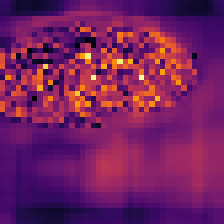
\includegraphics[width=0.13\textwidth]{resources/230916_1943_fig1_attmaps_before_after_100cc/clip_4reg_218_norms.png} &
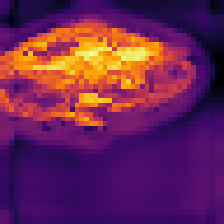
\includegraphics[width=0.13\textwidth]{resources/230916_1943_fig1_attmaps_before_after_100cc/dinov2_4reg_218_norms.png} \\

\includegraphics[width=0.13\textwidth]{resources/230916_1943_fig1_attmaps_before_after_100cc/219_orig.png} &
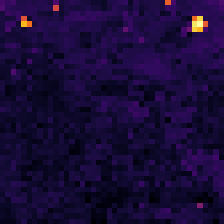
\includegraphics[width=0.13\textwidth]{resources/230916_1943_fig1_attmaps_before_after_100cc/deit3_0reg_219_norms.png} &
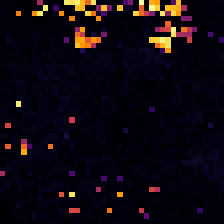
\includegraphics[width=0.13\textwidth]{resources/230916_1943_fig1_attmaps_before_after_100cc/clip_0reg_219_norms.png} &

\includegraphics[width=0.13\textwidth]{resources/230916_1943_fig1_attmaps_before_after_100cc/dinov2_0reg_219_norms.png} &
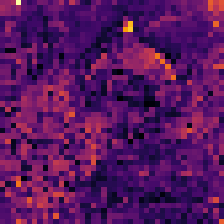
\includegraphics[width=0.13\textwidth]{resources/230916_1943_fig1_attmaps_before_after_100cc/deit3_4reg_219_norms.png} &
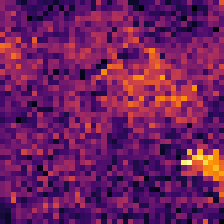
\includegraphics[width=0.13\textwidth]{resources/230916_1943_fig1_attmaps_before_after_100cc/clip_4reg_219_norms.png} &
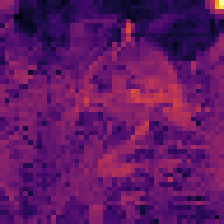
\includegraphics[width=0.13\textwidth]{resources/230916_1943_fig1_attmaps_before_after_100cc/dinov2_4reg_219_norms.png} \\
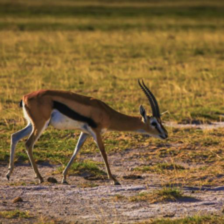
\includegraphics[width=0.13\textwidth]{resources/230916_1943_fig1_attmaps_before_after_100cc/242_orig.png} &
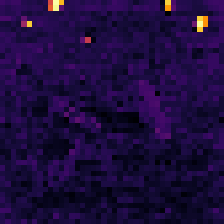
\includegraphics[width=0.13\textwidth]{resources/230916_1943_fig1_attmaps_before_after_100cc/deit3_0reg_242_norms.png} &
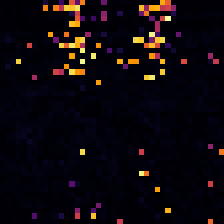
\includegraphics[width=0.13\textwidth]{resources/230916_1943_fig1_attmaps_before_after_100cc/clip_0reg_242_norms.png} &
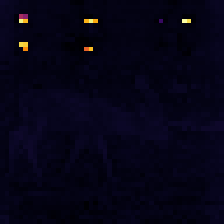
\includegraphics[width=0.13\textwidth]{resources/230916_1943_fig1_attmaps_before_after_100cc/dinov2_0reg_242_norms.png} &
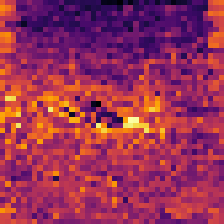
\includegraphics[width=0.13\textwidth]{resources/230916_1943_fig1_attmaps_before_after_100cc/deit3_4reg_242_norms.png} &
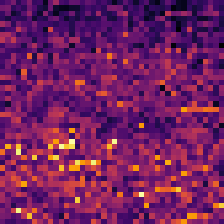
\includegraphics[width=0.13\textwidth]{resources/230916_1943_fig1_attmaps_before_after_100cc/clip_4reg_242_norms.png} &
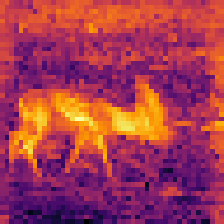
\includegraphics[width=0.13\textwidth]{resources/230916_1943_fig1_attmaps_before_after_100cc/dinov2_4reg_242_norms.png} \\

\includegraphics[width=0.13\textwidth]{resources/230916_1943_fig1_attmaps_before_after_100cc/285_orig.png} &
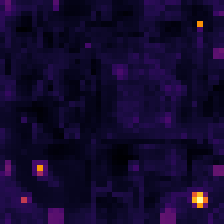
\includegraphics[width=0.13\textwidth]{resources/230916_1943_fig1_attmaps_before_after_100cc/deit3_0reg_285_norms.png} &
\includegraphics[width=0.13\textwidth]{resources/230916_1943_fig1_attmaps_before_after_100cc/clip_0reg_285_norms.png} &
\includegraphics[width=0.13\textwidth]{resources/230916_1943_fig1_attmaps_before_after_100cc/dinov2_0reg_285_norms.png} &
\includegraphics[width=0.13\textwidth]{resources/230916_1943_fig1_attmaps_before_after_100cc/deit3_4reg_285_norms.png} &
\includegraphics[width=0.13\textwidth]{resources/230916_1943_fig1_attmaps_before_after_100cc/clip_4reg_285_norms.png} &
\includegraphics[width=0.13\textwidth]{resources/230916_1943_fig1_attmaps_before_after_100cc/dinov2_4reg_285_norms.png} \\
\includegraphics[width=0.13\textwidth]{resources/230916_1943_fig1_attmaps_before_after_100cc/405_orig.png} &
\includegraphics[width=0.13\textwidth]{resources/230916_1943_fig1_attmaps_before_after_100cc/deit3_0reg_405_norms.png} &
\includegraphics[width=0.13\textwidth]{resources/230916_1943_fig1_attmaps_before_after_100cc/clip_0reg_405_norms.png} &
\includegraphics[width=0.13\textwidth]{resources/230916_1943_fig1_attmaps_before_after_100cc/dinov2_0reg_405_norms.png} &
\includegraphics[width=0.13\textwidth]{resources/230916_1943_fig1_attmaps_before_after_100cc/deit3_4reg_405_norms.png} &
\includegraphics[width=0.13\textwidth]{resources/230916_1943_fig1_attmaps_before_after_100cc/clip_4reg_405_norms.png} &
\includegraphics[width=0.13\textwidth]{resources/230916_1943_fig1_attmaps_before_after_100cc/dinov2_4reg_405_norms.png} \\
\includegraphics[width=0.13\textwidth]{resources/230916_1943_fig1_attmaps_before_after_100cc/512_orig.png} &
\includegraphics[width=0.13\textwidth]{resources/230916_1943_fig1_attmaps_before_after_100cc/deit3_0reg_512_norms.png} &
\includegraphics[width=0.13\textwidth]{resources/230916_1943_fig1_attmaps_before_after_100cc/clip_0reg_512_norms.png} &
\includegraphics[width=0.13\textwidth]{resources/230916_1943_fig1_attmaps_before_after_100cc/dinov2_0reg_512_norms.png} &
\includegraphics[width=0.13\textwidth]{resources/230916_1943_fig1_attmaps_before_after_100cc/deit3_4reg_512_norms.png} &
\includegraphics[width=0.13\textwidth]{resources/230916_1943_fig1_attmaps_before_after_100cc/clip_4reg_512_norms.png} &
\includegraphics[width=0.13\textwidth]{resources/230916_1943_fig1_attmaps_before_after_100cc/dinov2_4reg_512_norms.png} \\
\includegraphics[width=0.13\textwidth]{resources/230916_1943_fig1_attmaps_before_after_100cc/513_orig.png} &
\includegraphics[width=0.13\textwidth]{resources/230916_1943_fig1_attmaps_before_after_100cc/deit3_0reg_513_norms.png} &
\includegraphics[width=0.13\textwidth]{resources/230916_1943_fig1_attmaps_before_after_100cc/clip_0reg_513_norms.png} &
\includegraphics[width=0.13\textwidth]{resources/230916_1943_fig1_attmaps_before_after_100cc/dinov2_0reg_513_norms.png} &
\includegraphics[width=0.13\textwidth]{resources/230916_1943_fig1_attmaps_before_after_100cc/deit3_4reg_513_norms.png} &
\includegraphics[width=0.13\textwidth]{resources/230916_1943_fig1_attmaps_before_after_100cc/clip_4reg_513_norms.png} &
\includegraphics[width=0.13\textwidth]{resources/230916_1943_fig1_attmaps_before_after_100cc/dinov2_4reg_513_norms.png} \\
\includegraphics[width=0.13\textwidth]{resources/230916_1943_fig1_attmaps_before_after_100cc/532_orig.png} &
\includegraphics[width=0.13\textwidth]{resources/230916_1943_fig1_attmaps_before_after_100cc/deit3_0reg_532_norms.png} &
\includegraphics[width=0.13\textwidth]{resources/230916_1943_fig1_attmaps_before_after_100cc/clip_0reg_532_norms.png} &
\includegraphics[width=0.13\textwidth]{resources/230916_1943_fig1_attmaps_before_after_100cc/dinov2_0reg_532_norms.png} &
\includegraphics[width=0.13\textwidth]{resources/230916_1943_fig1_attmaps_before_after_100cc/deit3_4reg_532_norms.png} &
\includegraphics[width=0.13\textwidth]{resources/230916_1943_fig1_attmaps_before_after_100cc/clip_4reg_532_norms.png} &
\includegraphics[width=0.13\textwidth]{resources/230916_1943_fig1_attmaps_before_after_100cc/dinov2_4reg_532_norms.png} \\
\includegraphics[width=0.13\textwidth]{resources/230916_1943_fig1_attmaps_before_after_100cc/552_orig.png} &
\includegraphics[width=0.13\textwidth]{resources/230916_1943_fig1_attmaps_before_after_100cc/deit3_0reg_552_norms.png} &
\includegraphics[width=0.13\textwidth]{resources/230916_1943_fig1_attmaps_before_after_100cc/clip_0reg_552_norms.png} &
\includegraphics[width=0.13\textwidth]{resources/230916_1943_fig1_attmaps_before_after_100cc/dinov2_0reg_552_norms.png} &
\includegraphics[width=0.13\textwidth]{resources/230916_1943_fig1_attmaps_before_after_100cc/deit3_4reg_552_norms.png} &
\includegraphics[width=0.13\textwidth]{resources/230916_1943_fig1_attmaps_before_after_100cc/clip_4reg_552_norms.png} &
\includegraphics[width=0.13\textwidth]{resources/230916_1943_fig1_attmaps_before_after_100cc/dinov2_4reg_552_norms.png} \\
\includegraphics[width=0.13\textwidth]{resources/230916_1943_fig1_attmaps_before_after_100cc/553_orig.png} &
\includegraphics[width=0.13\textwidth]{resources/230916_1943_fig1_attmaps_before_after_100cc/deit3_0reg_553_norms.png} &
\includegraphics[width=0.13\textwidth]{resources/230916_1943_fig1_attmaps_before_after_100cc/clip_0reg_553_norms.png} &
\includegraphics[width=0.13\textwidth]{resources/230916_1943_fig1_attmaps_before_after_100cc/dinov2_0reg_553_norms.png} &
\includegraphics[width=0.13\textwidth]{resources/230916_1943_fig1_attmaps_before_after_100cc/deit3_4reg_553_norms.png} &
\includegraphics[width=0.13\textwidth]{resources/230916_1943_fig1_attmaps_before_after_100cc/clip_4reg_553_norms.png} &
\includegraphics[width=0.13\textwidth]{resources/230916_1943_fig1_attmaps_before_after_100cc/dinov2_4reg_553_norms.png} \\

    \end{tabular}
    }
    \caption{
        Maps of token norms for models trained without and with registers on various images.
        The norm outliers are very visible for models trained without registers.
        }
    \label{fig:supmat_pagefig_norms_beforeafter}
  \end{figure}








